\documentclass[10pt,xcolor=pdflatex,hyperref={unicode}]{beamer}
\usepackage{newcent}
\usepackage[utf8]{inputenc}
%\usepackage[czech]{babel}
%\usepackage[T1]{fontenc}
\usepackage{hyperref}
\usepackage{fancyvrb}
\usetheme{FIT}

\usepackage{setspace}
\usepackage{enumerate}
\usepackage[export]{adjustbox}
\usepackage{wrapfig}
%%%%%%%%%%%%%%%%%%%%%%%%%%%%%%%%%%%%%%%%%%%%%%%%%%%%%%%%%%%%%%%%%%
\title{Block Cleaning Application\\
(an10)}

\author[]{
Beránek Tomáš, Buchta Martin,\\
Klem Richard, Pešková Daniela}

\institute[]{Brno University of Technology, Faculty of Information Technology\\
Bo\v{z}et\v{e}chova 1/2. 612 66 Brno - Kr\'alovo Pole}


% České logo - Czech logo
% beamerouterthemeFIT.sty řádek 9: fitlogo1_cz

\date{\today}
%\date{} % bez data / without date

%%%%%%%%%%%%%%%%%%%%%%%%%%%%%%%%%%%%%%%%%%%%%%%%%%%%%%%%%%%%%%%%%%

\begin{document}


\frame[plain]{\titlepage}


\begin{frame}\frametitle{Project goal}
    \begin{itemize}
        \item Notify you about upcoming block cleaning
        \vspace{0.25cm}
        \item Gather data from all Brno districts
        \vspace{0.5cm}
    \end{itemize}
    
    \begin{center}
        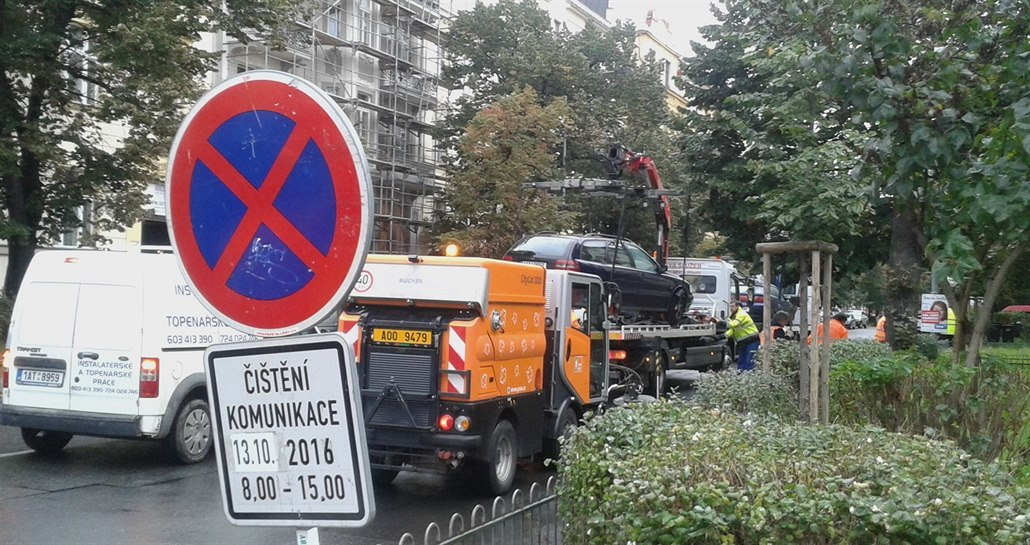
\includegraphics[width=0.65\paperwidth]{img/block-cleaning-1.jpg}
    \end{center}
\end{frame}


\begin{frame}\frametitle{What's done}
    \begin{itemize}
        \item Fetching data from API
        \item Basic project skeleton
        \item Responsive UI
        \item Dynamic map - in progress
        \item UI connection with API - in progress
    \end{itemize}
\end{frame}


\begin{frame}\frametitle{Wireframes}
    \begin{figure}
        \centering
        \begin{minipage}{0.3\textwidth}
            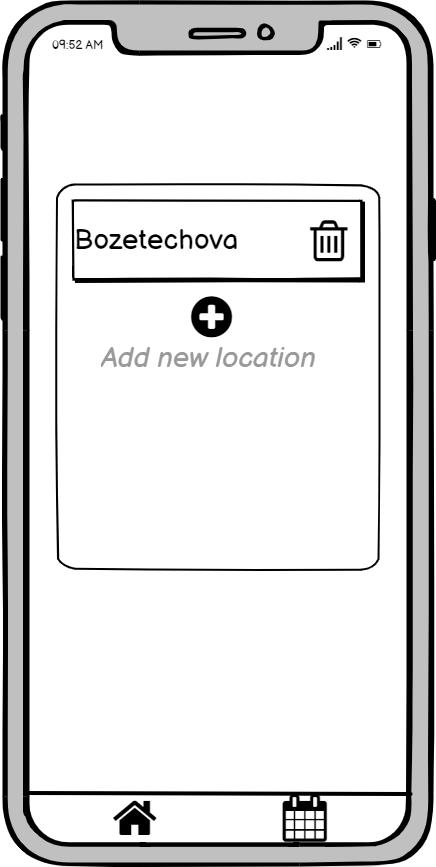
\includegraphics[width=0.25\paperwidth]{img/wireframe1.png}
        \end{minipage}
        \hfill
        \begin{minipage}{0.3\textwidth}
            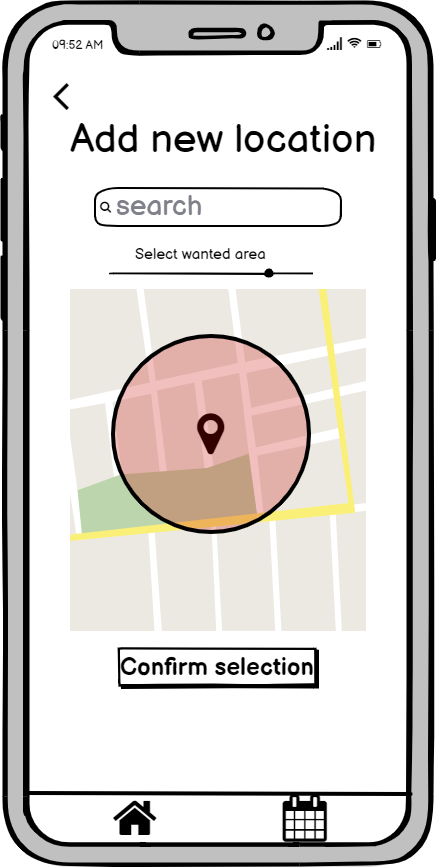
\includegraphics[width=0.25\paperwidth]{img/wireframe2.png}
        \end{minipage}
        \hfill
        \begin{minipage}{0.3\textwidth}
            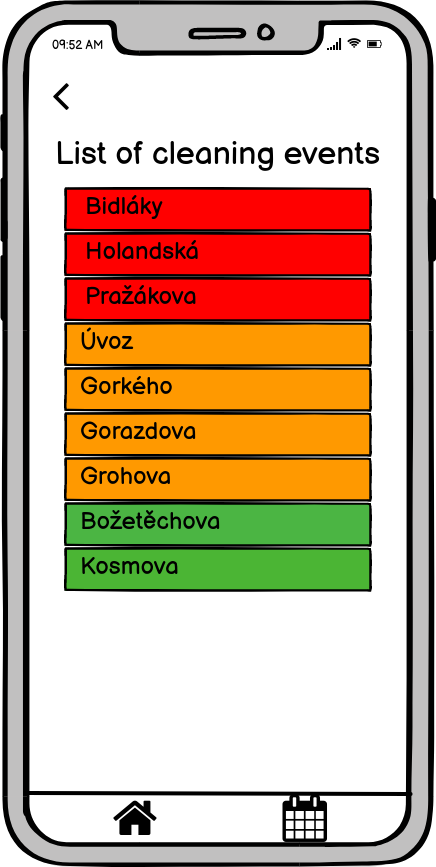
\includegraphics[width=0.25\paperwidth]{img/wireframe3.png}
        \end{minipage}
    \end{figure}
\end{frame}


\begin{frame}\frametitle{UI prototype}
    \begin{figure}
        \centering
        \begin{minipage}{0.3\textwidth}
            \centering
            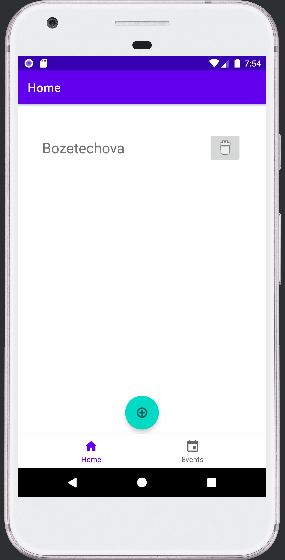
\includegraphics[width=0.25\paperwidth]{img/ui1.jpg}
        \end{minipage}
        \hfill
        \begin{minipage}{0.3\textwidth}
            \centering
            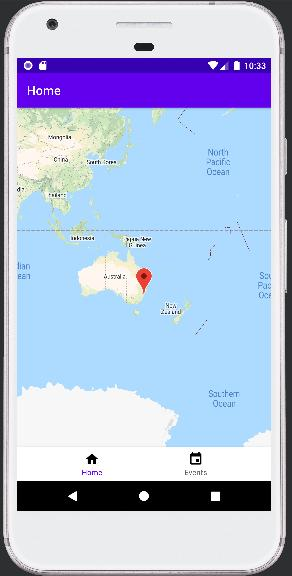
\includegraphics[width=0.25\paperwidth]{img/ui2.jpg}
        \end{minipage}
        \hfill
        \begin{minipage}{0.3\textwidth}
            \centering
            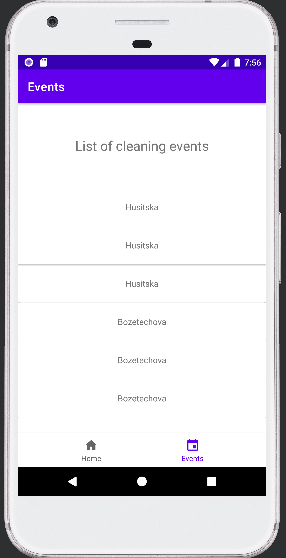
\includegraphics[width=0.25\paperwidth]{img/ui3.jpg}
        \end{minipage}
        \hfill
    \end{figure}
\end{frame}


\begin{frame}\frametitle{Time Plan}
    \begin{itemize}
        \item[] \textcolor{blue}{Oct 4} -- Wireframes, presentation for Project Workshop
        \item[] \textcolor{blue}{Oct 5} -- Project Workshop
        \item[] \textcolor{blue}{Oct 10} -- Agreeing on the technologies to be used
        \item[] \textcolor{blue}{Oct 17} -- Creating a basic UI
        \item[] \textcolor{blue}{Oct 25} -- Data fetching
        \item[] \textcolor{blue}{Oct 26} -- Project Workshop
        \item[] \textcolor{blue}{Nov 7}  -- Adding a dynamic map
        \item[] \textcolor{blue}{Nov 12} -- Connect UI with the data from API
        \item[] \textcolor{blue}{Nov 14} -- Functionality testing and documentation
        \item[] \textcolor{blue}{Nov 16} -- Project Workshop
        \item[] \alert{Dec 7}  -- Project Workshop
        \item[] \alert{Dec 12} -- Project submission
        \item[] \alert{Dec 14} -- Project Workshop
    \end{itemize}
\end{frame}


\bluepage{Thank you for your attention}
\end{document}
